\documentclass[a4paper,12pt]{article}
\usepackage[hidelinks]{hyperref}
\usepackage{graphicx}
\usepackage{float}
\usepackage{caption}
\begin{document}
\begin{center}

%Cover page
\Huge\textbf{Requirements and Design Specification(uWatch digital forensic tool)\\}
																											
\vspace{2 cm}

\LARGE\textbf{Group Name:} MPHETamines\newline
 
\LARGE\textbf{Version:} 1.2\newline
 
 
 
 
\vspace{0.5 cm}
\begin{tabular}{lr}
Taariq Ghoord&10132806
\\ 
Martha Mohlala&10353403
\\
Phethile Mkhabela&12097561
\\
Sboniso Masilela&10416260
\\
Harrison Maphuti Setati&12310043\\
\end{tabular}

\vspace{1cm}
\textbf{Git repository link:\\}
\url{https://github.com/MPHETamines/MPHETamines/}

\vspace{1cm}
\textbf{\today}
\end{center}
\pagenumbering{gobble}
\newpage

%table of contents
\tableofcontents

\newpage
\pagenumbering{arabic}

\section{Introduction}
This document sets out the Software Requirements Specification and Technology Neutral Process Design for the COS 301 group project entitled \textit{Online Neighbourhood Watch(ONW aka uWatch)}.
The aim for this project is to follow agile software development approach within which the application functionality is developed 
iteratively. 
The information provided in this document is presented in such a way as to provide precise and testable requirements. The emphasis is on performing an upfront software 
architecture engineering for iterative stimulation of the detailed requirements for a use case so that each use case can be built, tested and deployed before the detailed 
requirements for the next case are added.
\subsection{Project Background}
Crime is a prominent issue in South Africa as it is all over the world, Many criminal activities go unresolved or even attended to due to the lack of evidence or concrete witnesses.  Mobile applications have become increasingly popular all over the world and are used in our everyday and work life for common things such as checking the weather; maps for directions and news feed updates.  Digital forensic science hopes to utilise this increasing growth in the use of mobile applications to address the lack of evidence to crime cases in South Africa.

The application is referred to as Online Neighbourhood Watch(ONW) accessible via mobile devices and computers over the internet.  The two main users of the ONW model are the uploader (user of the mobile device) and the forensic investigator or law enforcement agent. 
This tool is to be used by the citizens of South Africa to capture, collect and store potential evidence which can later be viewed and analysed by the Police department and used in the prosecution and detention of criminals.
\subsection{Project Purpose}
The Online Neighbourhood Watch is aimed to provide a tool that can assist the South African Police Services(SAPS) reduce crime by enabling the members of the community to be part of the judicial system.  The ONW application captures and stores potential digital evidence of criminal activities which will then be accessed by law enforcement agents and digital forensic investigators.  The goal is to enhance the successful rate of trials and secure a higher number of convictions.\newline
The application can be used in various scenarios, basically it should be used in any setting where a community member feels like a crime has been committed, it is then up to the ONW model to decide if the uploaded data is a potential crime scene. The application should enable a user to capture digital evidence such as digital photographs, audio and video of a potential crime scene in the domain of the ONW to maintain integrity of the data, the data is then stored into the ONW repository.
\subsection{Project Scope}
The scope of the ONW is focused on capturing three media types(image,video and audio).Users will capture and upload images,videos and audio as potential digital evidence(PDE). There are two aspects of the system the mobile application side, utilised by South African community members; the desktop side where a law enforcement agent logs in. The PDE is categorised by using tags with drop-down describing the kind of the crimes.Our project has these categories: murder,rape,violence,robbery,drugs and other(relevant crimes). The PDE is tagged with geo-location and time-stamp(that is for making the searching of evidence easier on the law enforcement side) and uploaded to the SAPS server.

\subsection{Project Assumptions}
The ONW will be tested around Pretoria Hatfield with the local SAPS precinct. If it passes the test then it will be progressed to other cities in Gauteng, eventually to the whole South Africa. 

\section{Methodology}
We will be following agile approach when conducting our project.This incremental approach allows us to test each of the small components of the system independently.
Changes in the requirements may be made in this approach so maybe our limitations changing in the implementation phase will not be a problem.
 

\section{Application requirements and design}
This section discusses for each module of the uWatch Digital Forensic Tool,the functional requirements
as well as the process designs for the use cases.
\subsection{ONW Application Module}
The Application module will provide services to capture PDE, that is capture images, record videos and record audio to serve as a potential evidence. The user will be notified when an evidence(PDE) is successfully uploaded to the law enforcement server.
\subsubsection{CapturePDE-Priority:critical}
\textbf{Service Contract}\newline
post-condition: The PDE is captured and added to the database.\newline
\textbf{Functional Requirement}\newline
A user should be able to capture media in any situation they feel that a crime has been committed.	\newline
\subsubsection{UploadPDE-Priority:critical}
\textbf{Service Contract}\newline
pre-condition: The valid PDE was captured.\newline
post-condition: The PDE is encrypted.\newline
\begin{figure}[H]
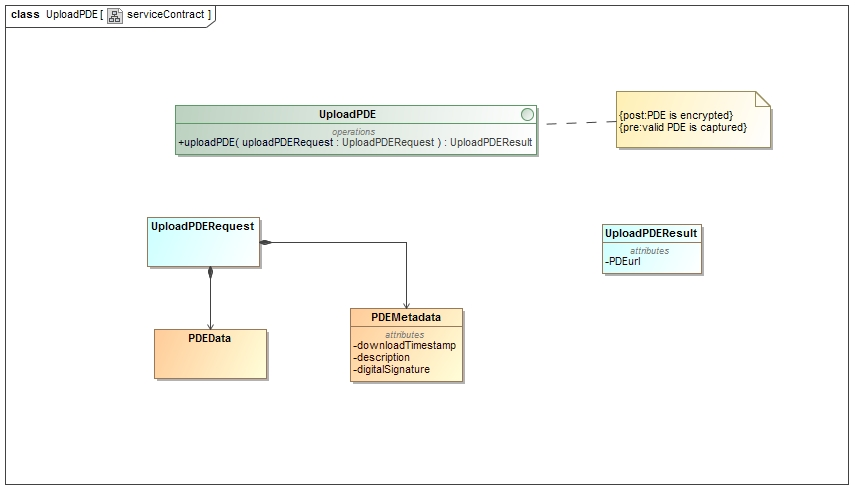
\includegraphics[width=\textwidth]{images/UploadserviceContract.jpg}
\caption{Service Contract: Uploading Potential Digital Evidence \label{overflow}}
\end{figure}\newpage
\textbf{Functional Requirement}\newline
A user needs to be able to upload a picture, video or audio whenever and wherever the user is.\newline

\begin{figure}[H]	
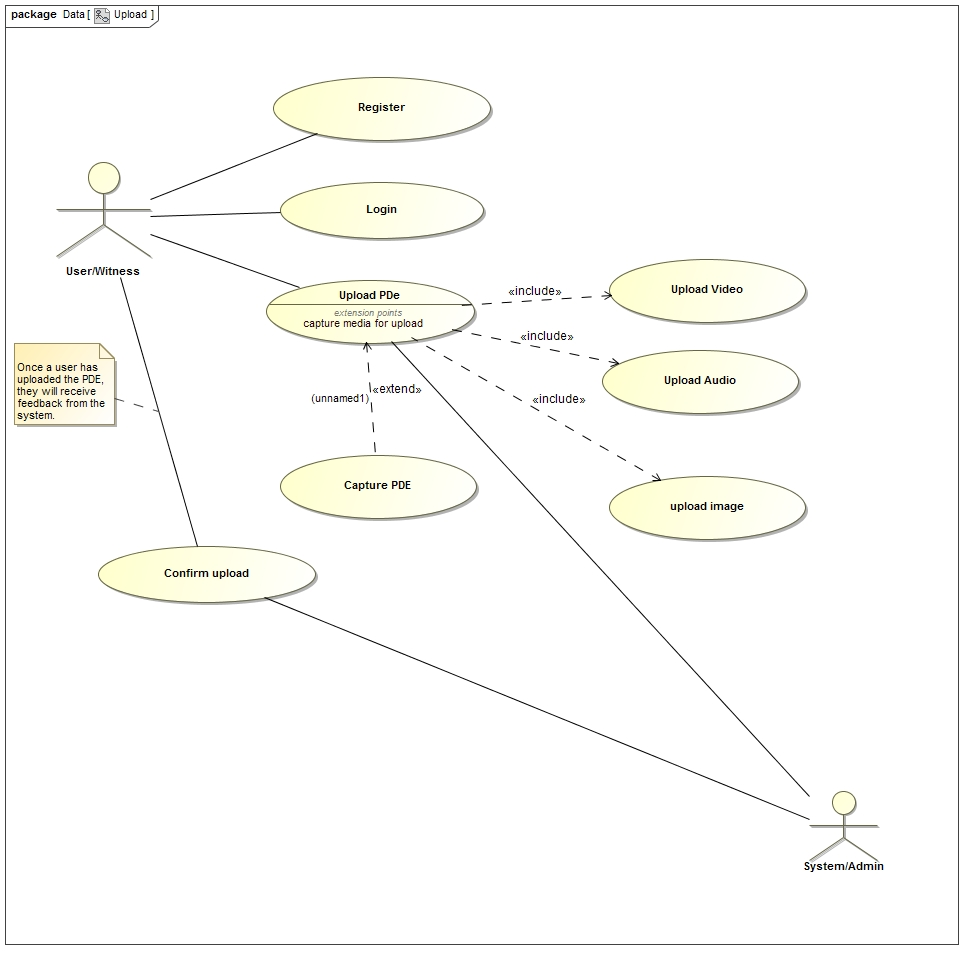
\includegraphics[width=\textwidth]{images/upload.jpg}
\caption{Functional Requirements: Uploading Potential Digital Evidence \label{overflow}}
\end{figure}
\begin{figure}[H]
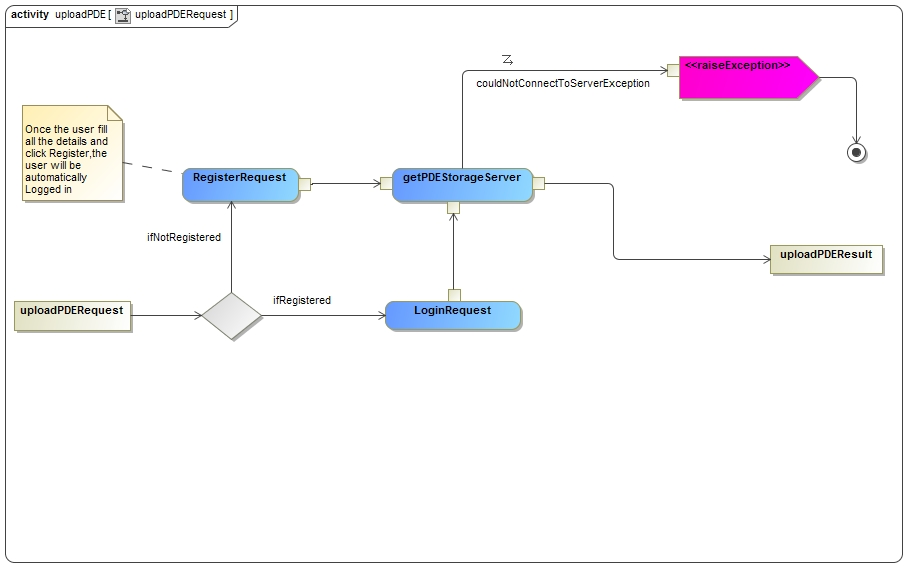
\includegraphics[width=\textwidth]{images/uploadPDERequest.jpg}
\caption{Process Specification: Uploading Potential Digital Evidence \label{overflow}}
\end{figure}
\subsubsection{ConfirmPDE-Priority:important}
\textbf{Service Contract}\newline
pre-condition: The user must have uploaded something to be confirmed.\newline
post-condition: The user gets a confirmation from the system.\newline
\textbf{Functional Requirement}\newline
The user waits to receive a confirmation from the system telling them if their PDE was accepted or rejected.\newpage
\subsection{The Administration Module}
The functionality provided by the Administration module includes the following:
\begin{itemize}
\item It manages access to the web based systems of the model
\item It provides means to download the potential digital evidence
\item It provides functionality to validate the evidence, whether by location, date and time or digital signature
\item It provides encryption and decrypt functionality
\end{itemize}
\subsubsection{DownloadPDE-Priority:critical}
\textbf{Service Contract}\newline
pre-condition: For any media to be downloaded, the media must be in the database.\newline
post-condition: The PDE must be persistent\newline
post-condition: The PDE is received\newline
\begin{figure}[H]
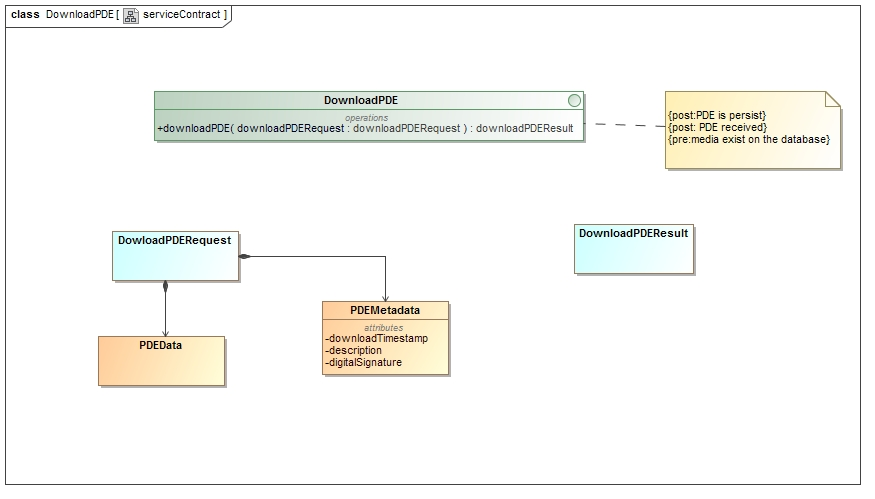
\includegraphics[width=1.0\textwidth]{images/downloadserviceContract.jpg}
\caption{Service Contract: Downloading Potential Digital Evidence \label{overflow}}
\end{figure}
\textbf{Functional Requirement}\newline
	The law enforcement agent needs to download the PDE to use it in the court of law. \newpage
\begin{figure}[H]
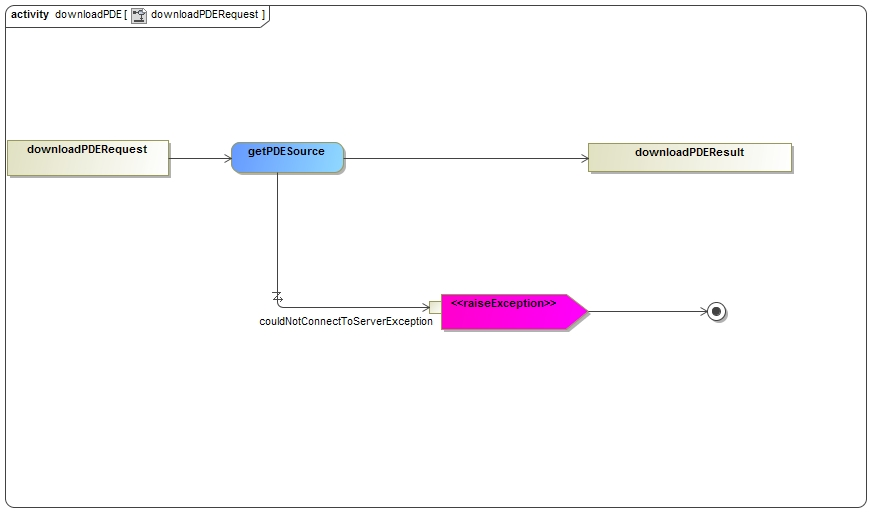
\includegraphics[width=\textwidth]{images/downloadPDERequest.jpg}
\caption{Process Specification: Downloading Potential Digital Evidence \label{overflow}}
\end{figure}	
\subsubsection{ValidatePDE-Priority:critical}
\textbf{Service Contract}\newline
post-condition: The PDE should be checked if it conforms to the standard set for valid evidence\newline
pre-condition: There has to be data to be validated\newline
\textbf{Functional Requirement}\newline
The system needs to validate that the data to ensure it's integrity.\newline
\subsubsection{EncryptPDE-Priority:critical}
\textbf{Service Contract}\newline
post-condition: The PDE should be encrypted.\newline
\textbf{Functional Requirement}\newline
	The system encrypts the PDE for it to be stored in the database.\newline
\subsubsection{DecryptPDE-Priority:critical}
\textbf{Service Contract}\newline
post-condition: The PDE should be decrypted before it is used in the court of law.\newline
\textbf{Functional Requirement}\newline
The system decrypts the PDE for it to be viewed in the court of law.\newline
\begin{figure}[H]
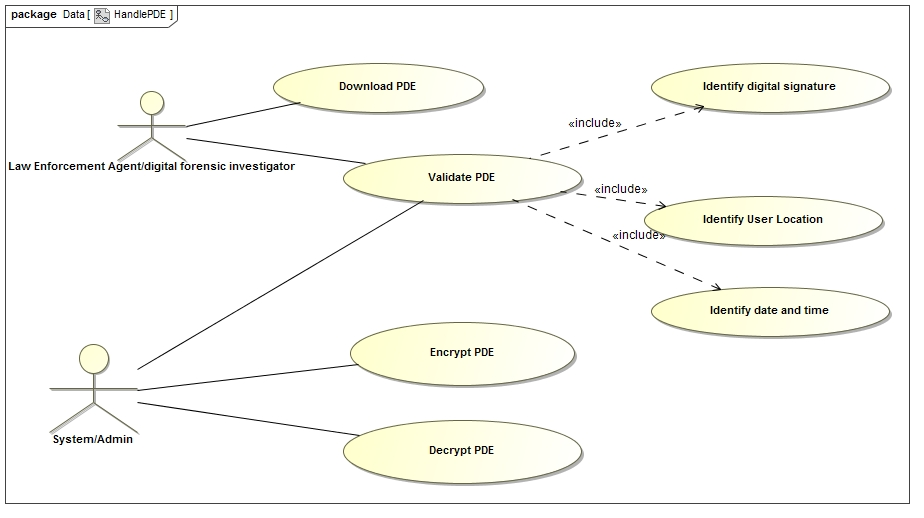
\includegraphics[width=\textwidth]{images/HandlePDE.jpg}
\caption{Functional Requirements: Validate,encrypt and decrypt PDE\label{overflow}}
\end{figure}
\subsubsection{ManageAccessAllocation-Priority:critical}
\textbf{Service Contract}\newline
post-condition: No unauthorised user can log in to the system.\newline
\textbf{Functional Requirement}\newline
The system is suppose to manage who has access to the system, this is a form of security measure. If the user is not authorized, he/she will be given an option to register new account.\newline
\begin{figure}[H]
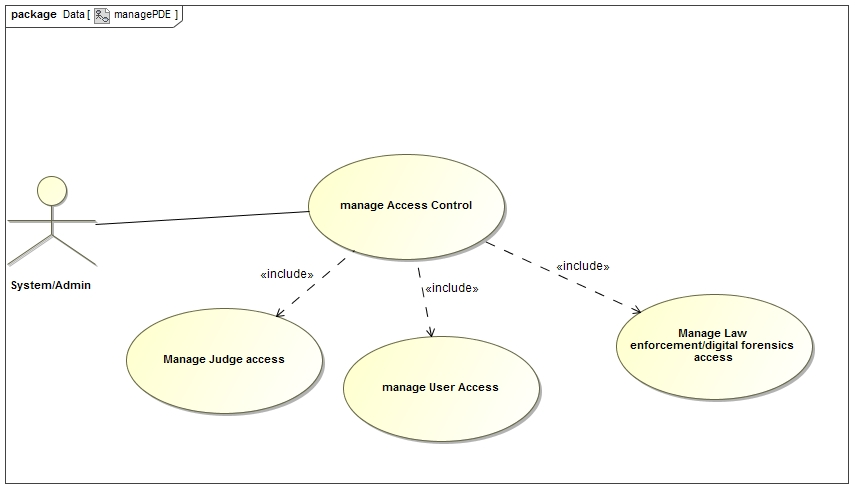
\includegraphics[width=\textwidth]{images/managePDE.jpg}
\caption{Functional Requirements: Manage Access Allocation\label{overflow}}
\end{figure}
\subsection{Login and Administrative user}
The system provides a functionality to register new users or to log on already registered users. 
The system will be running on a remote server and user details are stored in a relation database.\newline
The Login module provides services to log in. Once a user is logged in, the user can view all the files he/she has uploaded to the server without being able to download them.\newline

Administrators on the other end, will also be requested to log in to the system before they could view, download or audit data files send to the server. 
 
\subsubsection{Login-Priority:critical}
\textbf{Service Contract}\newline
pre-condition: law enforcement agent and jury with provided credentials can login.\newline
pre-condition: Could connect to the SAPS database.\newline
post-condition: UserID on results is populated by user's ID.\newline
\begin{figure}[H]
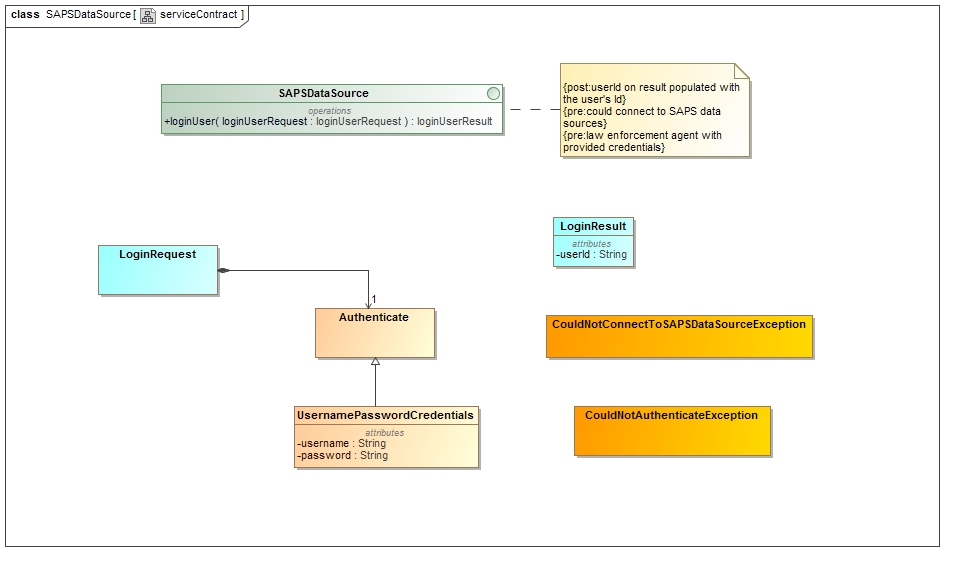
\includegraphics[width=\textwidth]{images/SAPSserviceContract.jpg}
\caption{Service Contract: Login for law enforcement and jury\label{overflow}}
\end{figure}\newpage
\textbf{Functional Requirement}\newline
The law enforcement agent should be able to log in to the system to search, view and download the PDE.\newline
\begin{figure}[H]
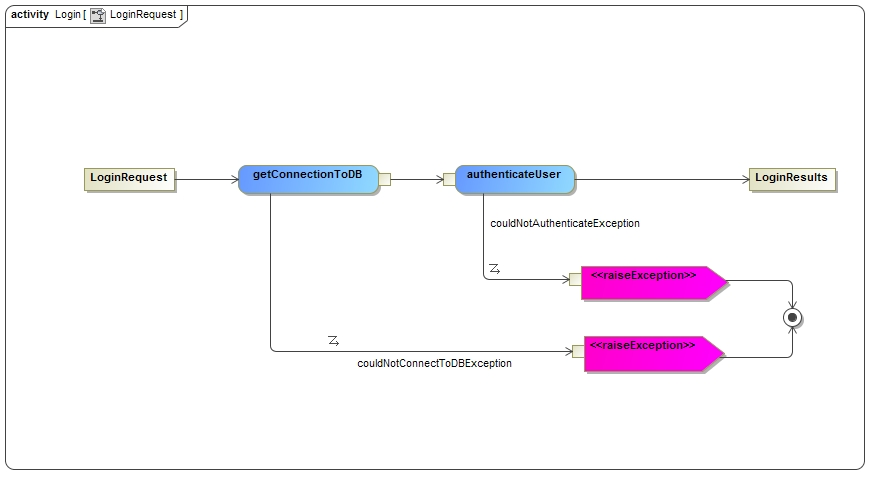
\includegraphics[width=\textwidth]{images/LoginRequest.jpg}
\caption{Process Specification: Login for law enforcement and jury\label{overflow}}
\end{figure}
\subsubsection{ViewPDE-Priority:important}
\textbf{Service Contract}\newline
pre-condition: The PDE is in the database to be viewed.\newline
post-condition: The law enforcement agent can view the PDE.\newline
\begin{figure}[H]
\includegraphics[width=\textwidth]{images/viewServiceContract.jpg}
\caption{Service Contract: View Potential Digital Evidence.\label{overflow}}
\end{figure}\newpage
\textbf{Functional Requirement}\newline
The law enforcement agents should be able to search, view, download and audit what has been uploaded to the server as evidence. They should also be able to see who has uploaded what and the contact details of the person who uploaded the file(s).\newline

\begin{figure}[H]
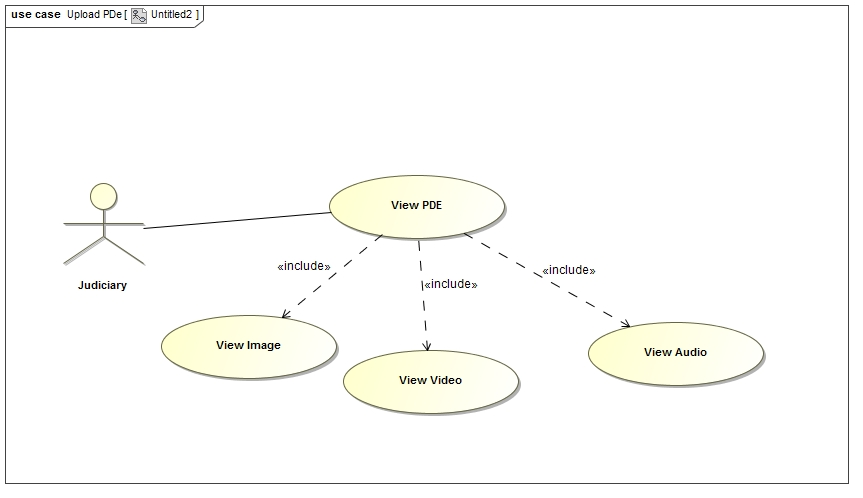
\includegraphics[width=\textwidth]{images/view.jpg}
\caption{Functional Requirements: View PDE\label{overflow}}
\end{figure}
\newpage
\subsection{Functionalities implemented}
\textbf{list of functionalities implemented from system's use cases:}
\begin{itemize}
	\item Geolocation: ability to detect the system's location at the time the evidence is captured.
	\item Detect internet connection: ability to tell whether there was internet connection when the evidence was captured.
	\item Capture PDE: ability to capture images, record audio and video as evidence with our system.
	\item Upload PDE: ability to send evidence to the database and retrieving it as needed.
	\item Search: ability for the law enforcement to search PDE file by tags.
	\item Download PDE: ability for the law enforcement to download pde.
	\item View PDE: ability for the users and law enforcement to view what has been uploaded
	\item Login and registration: ability for system users to login or register themselves in order to use the system.
	\item Access control: law enforcement and users have different rights levels

\end{itemize}

\textbf{Newly added functionalities:}
\begin{itemize}
	\item Battery status: This functionality ensures that users upload the evidence before the battery goes flat.
	\item Tagging: Tag every pde with the geographic location and the time stamp
	\item Two factor authentication: User get to verify the email address.
	\item One time password(OTP): user gets a one time password when they register new account.
	\item Theme: user can choose a theme for the look and feel of the mobile app.
\end{itemize}

\section{Architectural Requirements}
\subsection{Architectural scope}
This system integrate the back-end and the front-end. The front-end of the system is a hybrid mobile app which implements all the front end functionalities required. Functionalitites such as capture videos, audios and images and send those files to a server running on the back end. On the back-end the system runs Apache server, where all the large data files are stored, relational database, where user details and the links to where the files users uploaded. This front-end-back-end integration is made possible by PHP scripts on the server. The app makes RESTful request(http) to send files and user details upon registration to the server.  
\subsection{Quality requirements}
	\subsubsection{Security(core)}
	\begin{itemize}
		\item The system must prevent sql injection
			\begin{itemize}
				\item The system does string escaping and input validation
			\end{itemize}
		\item The system must verify user emails
			\begin{itemize}
				\item Upon registration, the user is send OTP to verify hi/her email address
			\end{itemize}
		\item The system must implement strong authentication
			\begin{itemize}
				\item Something user has and something user knows
			\end{itemize}
		\item The system must detect attacks from unwanted and unauthorized users.
			\begin{itemize}
				\item Prevent all unauthorized users from accessing the system 
			\end{itemize}
		\item The system must resist attacks from unwanted and unauthorized users.
			\begin{itemize}
				\item Ensure user's password is longer and strong
			\end{itemize}
		\item The system must recover from attack from unwanted and unauthorized users.
		
		\item The system must minimize access and permissions given to users who do not have the
			required privileges.
				\begin{itemize}
				\item Users can only capture and upload, they can not download what the have uploaded.
	 
			\end{itemize}
		\item All communication of sensitive data must be done securely through
			encryption and secure channels.
				\begin{itemize}
				\item Protect user's details and files they have uploaded
			\end{itemize}
		\item System ensures data integrity
				\begin{itemize}
				\item Ensure user's details and file are not tempered with 
			\end{itemize}
	\end{itemize}
	\subsubsection{Scalability(core)}
	\begin{itemize}
		\item The system operate effectively under a load of registered users.
		\item The system scales out resources.
		\item The system manages resource demand.
	\end{itemize}
	\subsubsection{Reliability(core)}
		\begin{itemize}
			\item The system must prevent faults.
			\item The system must detect faults.
			\item The system must recover from faults.
		\end{itemize}
	\subsubsection{Integrability(core)}
		\begin{itemize}
			\item The system must integrate with law enforcement server.
			\item The system integrate with Google maps for Geo-location.
		\end{itemize}
	\subsubsection{Performance(core)}
		\begin{itemize}
			\item Throughput:The rate at which incoming requests are completed.
			\item The system minimize the responsive time.
		\end{itemize}
	\subsubsection{Usability(core)}
		\begin{itemize}
			\item The system must be efficient.
			\item The system must be easy to use.
			\item The user must be satisfied by the system.
		\end{itemize}
	\subsubsection{Maintainability}
		\begin{itemize}
			\item System must be easy to be tested, updated and changed if needed.
		\end{itemize}
	\subsubsection{Deployability(important)}
		\begin{itemize}
			\item The system is deployed into cross platforms.
		\end{itemize}
\subsection{How we intend to achieve Quality requirements}
\subsubsection{Security}
	\begin{itemize}
		\item Access control: We have our own access control where registering users have different level of privileges. First of all,user has to login to view what he/she has uploaded and users can only view what they have uploaded. Law enforcement on the other hand, has privileges to view and download any pde uploaded by any user.
		\item 2 factor authentication - Every user has to confirm hi/her email address for him/her to be successfully registered.
		\item Hashing: We implement sha256 hash algorithm were we hash users passwords and links to pde before they are send to a cloud. 
		\item Encryption: We implement AES encryption algorithm. We encrypt users passwords and links to pde before the pde is sent to a cloud. 
		\item SSL: we use secure layers to connect to the database to ensure extra communication security when sending data and receiving it from the cloud and database.
	\end{itemize}
\subsubsection{Scalability}
	\begin{itemize}
		\item Data storage: We use both the database and the cloud to even up the load. We store users information in the database and user's pde files in the cloud and save the link of those large files in the database. This simplifies database structure and increases performance since the large data files are not queried to/from the database but only the partial link of the file is stored in the database and the file itself is stored in cloud. Every user has a related to a list of links of pde files he/she uploaded on our system. 
	\end{itemize}
\subsubsection{Reliability}
	\begin{itemize}
		\item Testing: We are using tested plugins from ngCordova repository to access device's camera, audio and video options. The plugins have been tested and we also do our own integration tests to ensure that the plugins work well with no conflicts.
		\item Exception handling: We catch all our exceptions to ensure that the system behaves as intended.
		\item Fault tolerance: A copy of the pde file is kept in our system cache until it is successfully uploaded to the cloud, in case there is a connection error while a user tries to upload the pde file. If there is an error, the cached pde file will be resend.  
	\end{itemize}
\subsubsection{Integrability}
	\begin{itemize}
		\item Our system is integrated with google map api to decode the longitude and latitude values we get from user's device location to human-readable address.
		\item Server: We integrate mysql database with Apache server to save large files on the server and store the link to the files on the database.
		\item Plugins: We integrate media plugins to access device's camera, audio and video controls with encryption and hashing algorithms. 
	\end{itemize}
\subsubsection{Performance}
	\begin{itemize}
		\item Cloud and Database: We separated user details from large files users upload to increase performance and to structure our data well.
	\end{itemize}
\subsubsection{Usability}
	\begin{itemize}
		\item Ionic framework build hybrid apps that uses native device's controls, meaning users enjoy the feel of using an app that is build with native language on any device the user will be using our system on. The button, forms and checkboxes feel as if they were build from native languages on both android and ios devices, meaning users will ship their knowledge of using the device and making it easier for users to adapt and learn to use the system quicker.
		\item Icon: We use visuals such as icons for users who can not even read to be able to still use the system because of the visuals on the buttons.
		\item Colors: We use colors to show users the quality and strength of their passwords, making them to enter the right secure password from the start.
	\end{itemize}
\subsubsection{Maintainability}
	\begin{itemize}
		\item MVC: We use MVC design pattern to separate the view from the controller and the model. This helps us modularize our system and make it easy to maintain and test it. 
		\item State pattern: Every view has it's state and depending on the state, a relevant page loads, this simplifies page linking and makes it easy to load any page dynamically depending on the stage of the current page or on which button pressed.   
	\end{itemize}
\subsubsection{Deployability}
	\begin{itemize}
		\item We are building a hybrid system that can be deployed in almost all the platforms. We are focusing on Android, Ios and windows mobile devices because of the higher percentage in the use of these devices. This also reduces the quirks of different devices and ensures reliability on every device and high performance.  
	\end{itemize}
\subsection{Integration and access channel requirements}
The system will be accessed using Mobile/Android Applications clients through the use of ngCordova,  browser clients which is where ionic's web based framework comes in and web services clients.
\subsection{Architectural constraints}
\begin{itemize}
\item There are multiple factors that may place constraints on the architecture that
is being developed for the uWatch System

\item This is developed under ionic framework which is simply web based, thus it put constraints on certain programming languages Compliance with existing standards
\end{itemize}
\section{Architectural pattern or styles}
		\subsection{MVC(Model-View-Controller)}
			\begin{itemize}
				\item Ionic framework is build from this pattern, where the view is the template HTML pages, the model is the JSON object to and from the database and the controller is the JavaScript functions to implement the system's functionality.
			\end{itemize}
		\subsection{Pipes and Filters}
		\begin{itemize}
		\item We will be tagging images, videos and audio files being uploaded to the server and using this architectural pattern to allow us to easily search and filter by tags and categorize the PDE being uploaded.
		\end{itemize}
		\subsection{Client/Server} 
			\begin{itemize}
				\item uWatch allows multiple clients to access the system using N-tier
				architectural style.The benefit of using N-tier architectural style is that
				it improves the scalability of the system.
				\item The server side is the back-end of the system which manages the centralized data and access to the database from the server. The aim of
having the back-end manages the data is to achieve higher security. 
			\end{itemize}
\section{Architectural tactics or strategies}
\subsection{Security:} We do not cache user credentials nor keep them in history. This forces users to login everytime they need to login to the our system.  Users have a limited amount of tries to login. 
\subsection{Maintainability and Flexibility:} Our views are templated, separating the view from the templates. Since our system relies on AngulaJS, we inject dependencies and as such the is Inversion of control (IoC).
\subsection{Perfomance:} We catch users' retried PDE so that the system can respond faster especially on slow internet connection. Localstorage caches data in case the relational DB goes down and once it goes up again, it synchronizes the cached data with the data in the DB.
\subsection{Scalability:} Our server is not tightly coupled with the system. The serve can be hosted any where, locally or remotely. Links to files stored on the server are send to a relation database.

We use local storage to store any PDE that the user chooses to upload later in case the user did not have internet connection at the time the PDE was captured.
\subsection{Reliability and Availability:} caching and local storage as explained above.
\subsection{Auditability :} Users login before they can upload a PDE. We use date, time-stamps and Geo-location.Data that is send to and from the serve is encrypted.
\subsection{Testing:}we will implement unit testing and integration tests to see if the pre and post condition are/were met.
\subsection{Usability:} We use nice icon and buttons and less text and encourage users who can not read to be able to use our system. Since it is a web base, we develop our system in away that blind and visual impaired users will be able to use screen readers to access our services.
\subsection{Integrability:} Our system is integratable since it is decoupled form the cloud/database, it can work with any database or a cloud for that matters or simply a local storage. 
\subsection{Deployability:} The system is cross platform, it will be deployable on IOS, Android, Windows, Amazon and blackberry platforms.	
\section{Use of reference architecture and frameworks}
\begin{itemize}
	\item We are using Ionic framework to implement our mobile application. Ionic framework is a mobile base 			framework build on the following frameworks:
	\begin{itemize}
		\item ngCordova – An Apache cordova framework which packages HTML, css and js files in to respective platform such as Android, IOS, Blackberry, Windows mobile etc.
		\item AngulaJS – Is a Google JavaScript framework that helps implement controllers and services 				for our project.
		\item Bower and Node package manager (NPM) to help install dependencies and plugins into our 		project in order for us to extend functionality beyond your normal JS capabilities.
		\item UI-Routes – we use routes to changes from one view to the other and from one state to another, this framework help us achieve exactly that.
		\item Gulp js – for simplifying our project and stripping out all unnecessary comments on our codes so that it can compile faster and respond quicker. Furthermore, the packaged final project file is relatively smaller and making it easy to deploy, share or to store.
		\item  SASS – this is the framework that deals with the look and feel of our application. SASS is described as css on steroid on the sass website.
	\end{itemize}
\item Reasons for choosing ionic framework:
	\begin{itemize}
		\item Since it is a web based, it leverages our web development skills and the knowledge we have of the web based languages such as js, HTML and css.
		\item It is cross platform, one project will be deployed on every platform. Meaning we do not need to write special code to accommodate a specific platform or learn the native language that each platform uses. This speeds up production and is convenient since we can not assume that users will be using one specific platform.
\item It is pretty powerful. We use ngCordova’s plugins to access native device camera, video camera, audio recording, media file, local storage etc… All this is done effortless.
\item Our app has to access one’s Geo-location and it is relatively easy to that with ionic than will a native language.
\item Is easy to implement security features in javascript
\item Is easier to debug, you can also debug in a browser’s console.
\item It uses less resources, you do not need an emulator to test features such as Geo-location or encryption
\item There are many encryption js libraries. For example forgejs, cryptojs and they both implement AES cryptography.
\item It's easy to work with JSON object.
\item It has a great community and up to date plugins.
	\end{itemize}
\end{itemize}
\section{Access and integration channels}
\begin{itemize}
\item Integration channels that we using:
\item We using a REST API which uses the Library cURL(which is a computer software project providing a library and command-line tool for transferring data using various protocols)

\item This REST API uses : 
\begin{itemize}
\item HTTPS (Hypertext Transfer Protocol Secure) is a protocol that allows safe and secure transfer of data over a network.
\item HTTP PUT for retrieving, writing and updating of data.
\end{itemize}

\item API specifications used in the integration of the systems
\begin{itemize}
\item Authentication API - We have our own access control were users are required to verify their email address by OTP
\item Security API - which an API that specifies rules(read,write and validate),what the client can be able to access and what restricted to them and it provides encryption strategies,for example Forge(which is an encryption method).
\end{itemize}

\item Quality requirements that can be achieved through the implementation of the access channels mentioned.
\begin{itemize}
\item Reliability so that the system is online as much as possible and that data transfer isn’t easily corruptible and that the transfer is fast. We use localstorage to back up the file before it is send to the server, if the file transfer fails or the file gets corrupted, then the local copy is tried until the file is successfully uploaded.

\item Security of user data being transferred.

\item Scalable so that a large amount of users data can be transferred to and from the systems.

\item Maintainable, the integration with the system must be easily maintained. (because for example security rules are all defined in one place.
\end{itemize}
\end{itemize}

\section{Technologies}
Technologies Used in the development of our Application are stated below along with why the choice was made and it's benefits.
\subsection{Ionic framework}
 \begin{itemize}
\item Ionic framework is a great framework that supports hybrid application which has many benefits, specifically in terms of access to third party code , speed development and  platform support.
\item It is an Model-View-Controller framework which separates concerns, allowing re-use of the business logic; it enables parallel development by separate teams which is ideal when working in a project such as this one.  The MVC framework uses AngularJS for controllers and services, HTML for view and JSON for the model which are all popular and easy to learn languages.
 \end{itemize}
\subsection{ngCordova}
\begin{itemize}
\item ngCordova is a collection of 63+ AngularJS extension on top of the cordova API that make it easy to build, test and deploy Cordova applications with AngularJS,  ngCordova uses packages and libraries, compiles source code and deploys the source code to Apk (android), Xap (windows mobile) and ipa (ios).
\end{itemize}
\textbf{Security provided by the serve includes:}
\begin{itemize}
\item Authentication API-who the user is.
\item Support SSL on all clients
\item Uses Bcrypt for password storage
\item Uses the JSON Web Token for standard credentials
\item Generate Server-Signed Tokens
\item All security Logic is put in one pace
\end{itemize}
 \textbf{The benefits of using PHP and MYSQL:}
\begin{itemize}
\item PHP has many libraries for encryption and hashing
\item Is easier to send email with php than with many server side language
\item PHP works well with session and tokens
\item MYSQL is easy to work with
\item Is easier to manage user details and writing sql queries 
\end{itemize}

\section{Unit testing}
Unit testing are done using karma and grunt. They support the following frameworks:
\begin{itemize}
\item Jasmine
\item Mocha
\end{itemize}
They support dependency injection and use angular-mocks for mock-up data.
\section{Integration testing}
Integration testing are done using grunt. Here no mocks are used.

\section{References}
\begin{itemize}
\item All About Ionic (author and date unknown) 
Available from:http://ionicframework.com/docs/guide
[Accessed: 31 july 2015]
\item Why use ngcordova (author and date unknown) 
Available from:http://stackoverflow.com/questions/31011051
[Accessed: 31 july 2015]
\item Features  (author and date unknown) 
[Accessed: 31 july 2015]
\item S.Omeleze,H.S.Venter, Toward a model for acquiring digital evidence using mobile devices. Information and Computer Security Architecture (ICSA) Research Group, University of Pretoria.
\item AGILE METHODOLOGY (author and date unknown)
	Available from: http://agilemethodology.org/ [Accessed: 15 May 2015]
\end{itemize}
\end{document}


